\section{Appendix}
\subsection{Example for a Small Delaunay Triangulation}
\label{appendix:DT_def}
    The Delaunay triangulation (DT) is an undirected graph. An edge
    between two nodes \(i\) and \(j\) will be drawn, if there exists
    a circle passing through \(i\) and \(j\), which does not contain
    any other node in its interior.
    \begin{figure}[htbp]
    \centering
        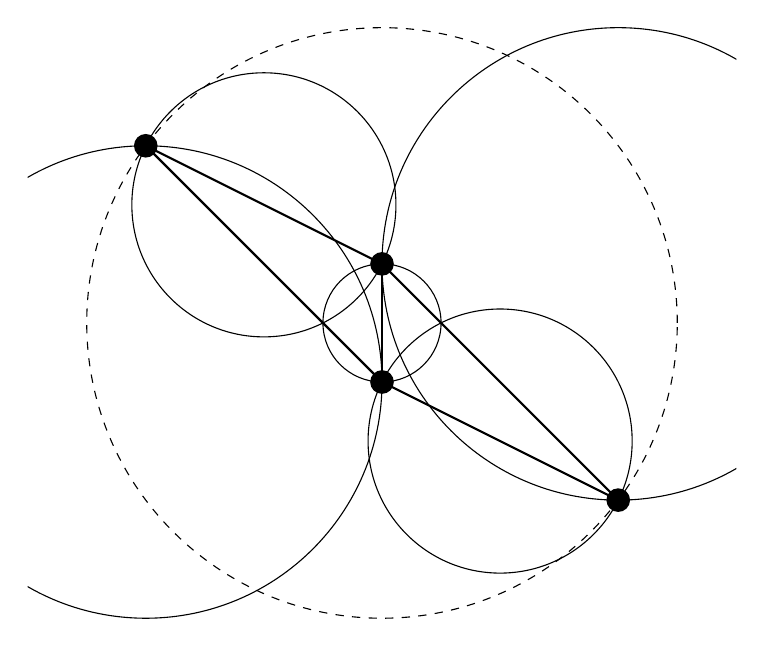
\begin{tikzpicture}[scale=3]
    \clip (-0.5,0) rectangle (2.5,2.5);

    \fill (0, 2  ) circle(0.05);
    \fill (1, 1.5) circle(0.05);
    \fill (1, 1  ) circle(0.05);
    \fill (2, 0.5) circle(0.05);

    \draw[dashed] (1, 1.25)   circle(1.25);
    \draw (2, 1.5)      circle(1);
    \draw (1, 1.25)     circle(0.25);
    \draw (0.5, 1.75)   circle(0.5590);
    \draw (1.5, 0.75)   circle(0.5590);
    \draw (0, 1)        circle(1);

    \draw[thick] (0, 2  ) -- (1, 1.5);
    \draw[thick] (0, 2  ) -- (1, 1  );
    \draw[thick] (1, 1  ) -- (1, 1.5);
    \draw[thick] (1, 1  ) -- (2, 0.5);
    \draw[thick] (1, 1.5) -- (2, 0.5);
\end{tikzpicture}

        \caption[Example for a Small Delaunay Triangulation]
        {
            Circles which contain nodes are dashed.
            Circles which contain no nodes are not dashed.
            Consequently nodes on the border of not dashed circles are
            connected. Note that the drawn cricles are only examples
            as there is an infinitive number of alternative not
            dashed circles which contain no other node.
            Note also that in contrast to the GG the circles do not
            have to be centered on the middle point between the nodes, if
            however the centered circle does not contain any node, the
            resulting edge will be present in DT and GG. Therefore GG is
            a subgraph of DT.
        }
        \label{fig:def:DT}
    \end{figure}

\subsection{Finite Size Effects at the Example of the Specific Heat}
\label{appendix:finiteSizeEffects}
    In Fig.\ \ref{fig:smeared_out_appendix}\subref{sfig:smeared_out_appendix:c} the specific heat
    \begin{equation}
        c = \frac{N}{T^2}\avg{\avg{E^2} - \avg{E}^2}
    \end{equation}
    is plotted for different system sizes. The finite size effects are obvious.
    The divergence is finite and gets steeper with larger \(L\). Besides
    the maximum moves to the critical temperature with larger \(L\).\\
    In Fig.\ \ref{fig:smeared_out_appendix}\subref{sfig:smeared_out_appendix:logL} the maxima of a
    cubic spline interpolation of \(c\) is plotted. Note that no errorbars
    are estimated. As mentioned before,
    this maximum increases logarithmically. One sees that a logarithmic
    fit is not worse than the power law fit. But to confirm the expected
    logarithmic growth, one would need much larger systems. Also the one
    would estimate the maximum by other means than an interpolation.
    \begin{figure}[htbp]
        \centering
        \subfigure[][]
        {
            \label{sfig:smeared_out_appendix:c}
            \includegraphics[width=0.45\textwidth]{plots/Specific_Heat_0}
        }
        \subfigure[][]
        {
            \label{sfig:smeared_out_appendix:logL}
            \includegraphics[width=0.45\textwidth]{plots/Specific_Heat_0_log}
        }
        \caption[Finite Size Effects by Example of the Specific Heat]
        {
            \subref{sfig:smeared_out_appendix:c} Effects of different system sizes on the specific heat \(c\)
            at \(\sigma = 0\). Dotted lines are guides to the eye.
            \subref{sfig:smeared_out_appendix:logL} maxima of \(c\) fitted
            with a power law function and a logarithm.
        }
        \label{fig:smeared_out_appendix}
    \end{figure}
